\documentclass{article}
\usepackage[margin=1in]{geometry}
\usepackage{graphicx}
\usepackage{hyperref}
\usepackage{enumitem}
\usepackage{float}
\usepackage{subfig}

\title{Education's Impact on Global Survival Rates: \\ A Narrative Visualization for Social Change}
\author{Sashank RM - sr6890}
\date{CS-GY 6313 B: Information Visualization}

\begin{document}
\maketitle

\section{Research Questions and Objectives}
Our visualization addresses three critical questions about global survival rates and educational impact:

\begin{enumerate}[label=\textbf{Q\arabic*.}]
    \item How do survival rates vary across different regions globally, and what role does educational access play in these variations?
    \item What is the magnitude of the survival gap between developed and developing nations?
    \item Can educational investment lead to improved survival rates in developing nations?
\end{enumerate}

\section{Design Rationale and Implementation}
\subsection{Visual Design Choices}
\begin{itemize}
    \item \textbf{Choropleth Map}:
        \begin{itemize}
            \item Blue-red diverging scale for intuitive interpretation of survival rates
            \item Dark blue ($>$90\%) indicates optimal outcomes
            \item Red tones ($<$70\%) highlight areas needing intervention
            \item Interactive tooltips provide precise values and context
        \end{itemize}
    \item \textbf{Time Series Visualization}:
        \begin{itemize}
            \item Line charts for clear trend visualization
            \item Consistent y-axis (50-100\%) for direct comparison
            \item Color-coded lines for country identification
            \item Interactive legend for dynamic filtering
        \end{itemize}
\end{itemize}

\section{Interactive Features}
\subsection{Core Interaction Methods}
\begin{enumerate}
    \item \textbf{Narrative Navigation}:
        \begin{itemize}
            \item Step-by-step guided tour through key insights
            \item Previous/Next controls for user-paced exploration
            \item Progress indicators showing narrative position
        \end{itemize}
    \item \textbf{Data Exploration Tools}:
        \begin{itemize}
            \item Year slider (2015-2021) for temporal analysis
            \item Country selection dropdown for comparative studies
            \item Linked views between map and trends
            \item Dynamic metric updates
        \end{itemize}
    \item \textbf{Information Access}:
        \begin{itemize}
            \item Hover tooltips with detailed statistics
            \item Click-through for detailed country analysis
            \item Dynamic insights panel with context
        \end{itemize}
\end{enumerate}

\section{Narrative Structure and Evidence}
\begin{figure}[H]
    \centering
    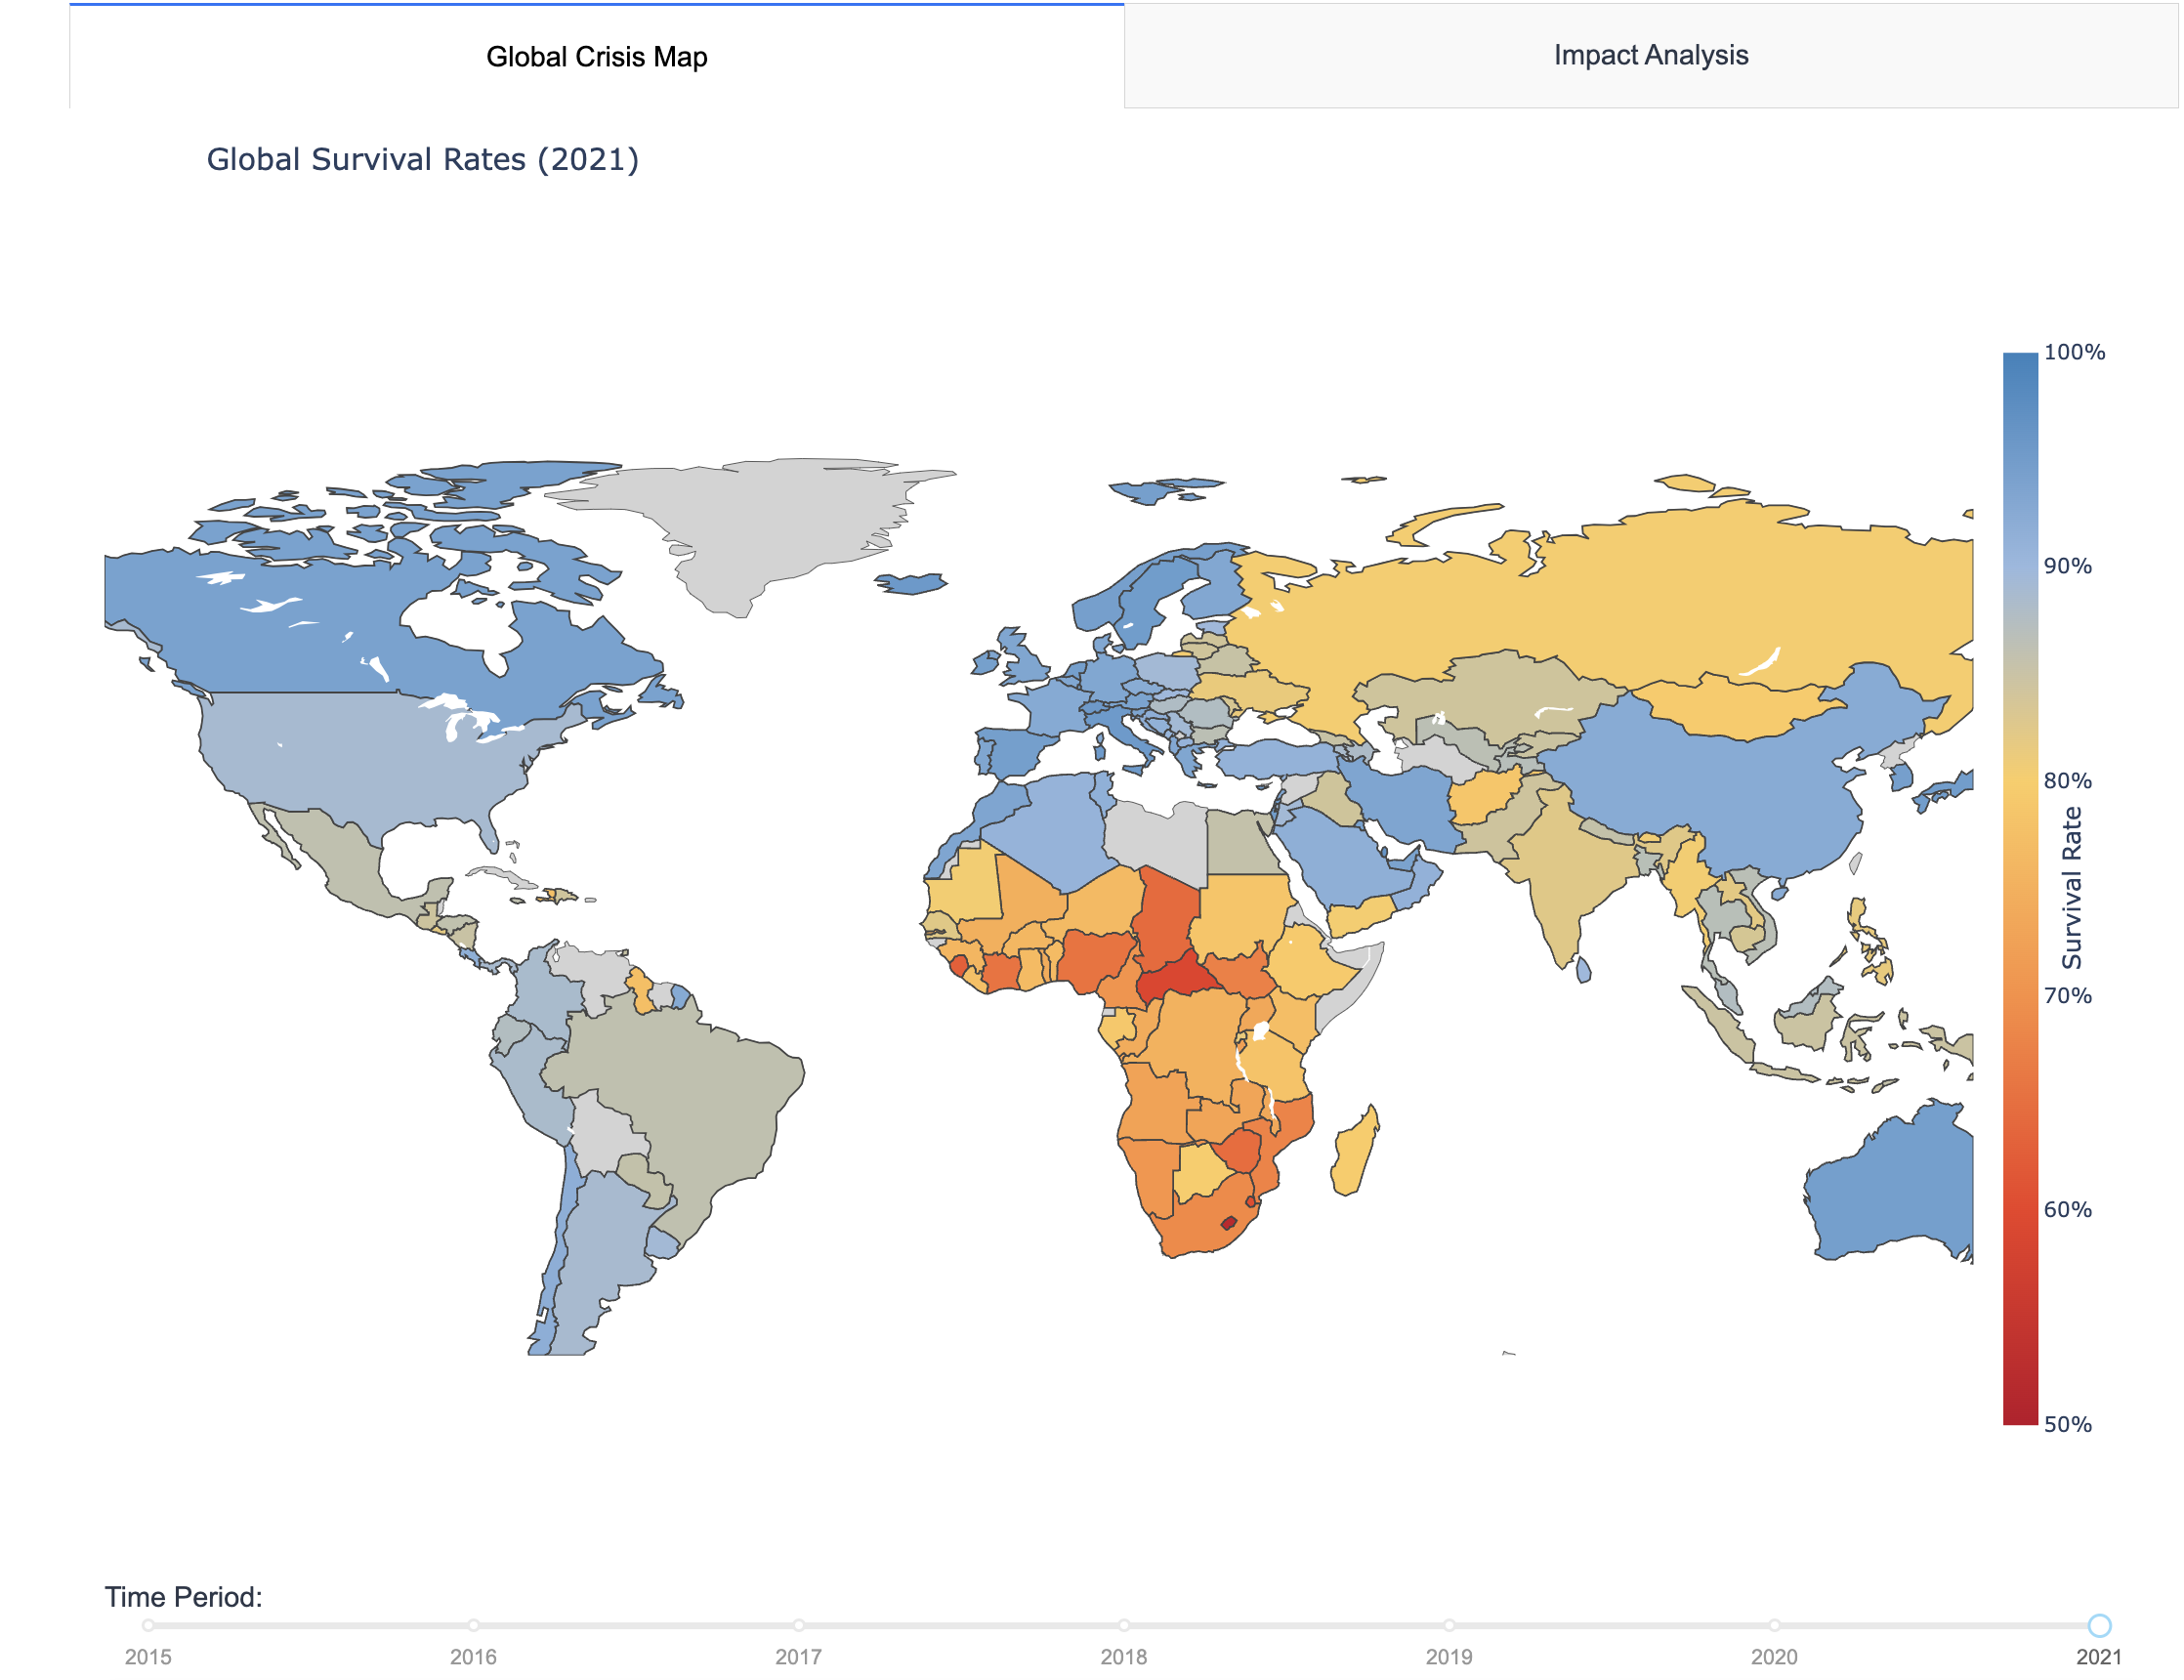
\includegraphics[width=\textwidth]{Global_map.png}
    \caption{Global Crisis Overview: Choropleth map revealing stark survival rate disparities (2021)}
    \label{fig:global_map}
\end{figure}

\subsection{Stage 1: Global Crisis Overview}
\begin{itemize}
    \item Map visualization reveals global survival rate patterns
    \item Clear north-south divide in outcomes
    \item Interactive features allow temporal exploration
    \item Color encoding highlights critical regions
\end{itemize}

\subsection{Stage 2: The Education-Survival Divide}
\begin{figure}[H]
    \centering
    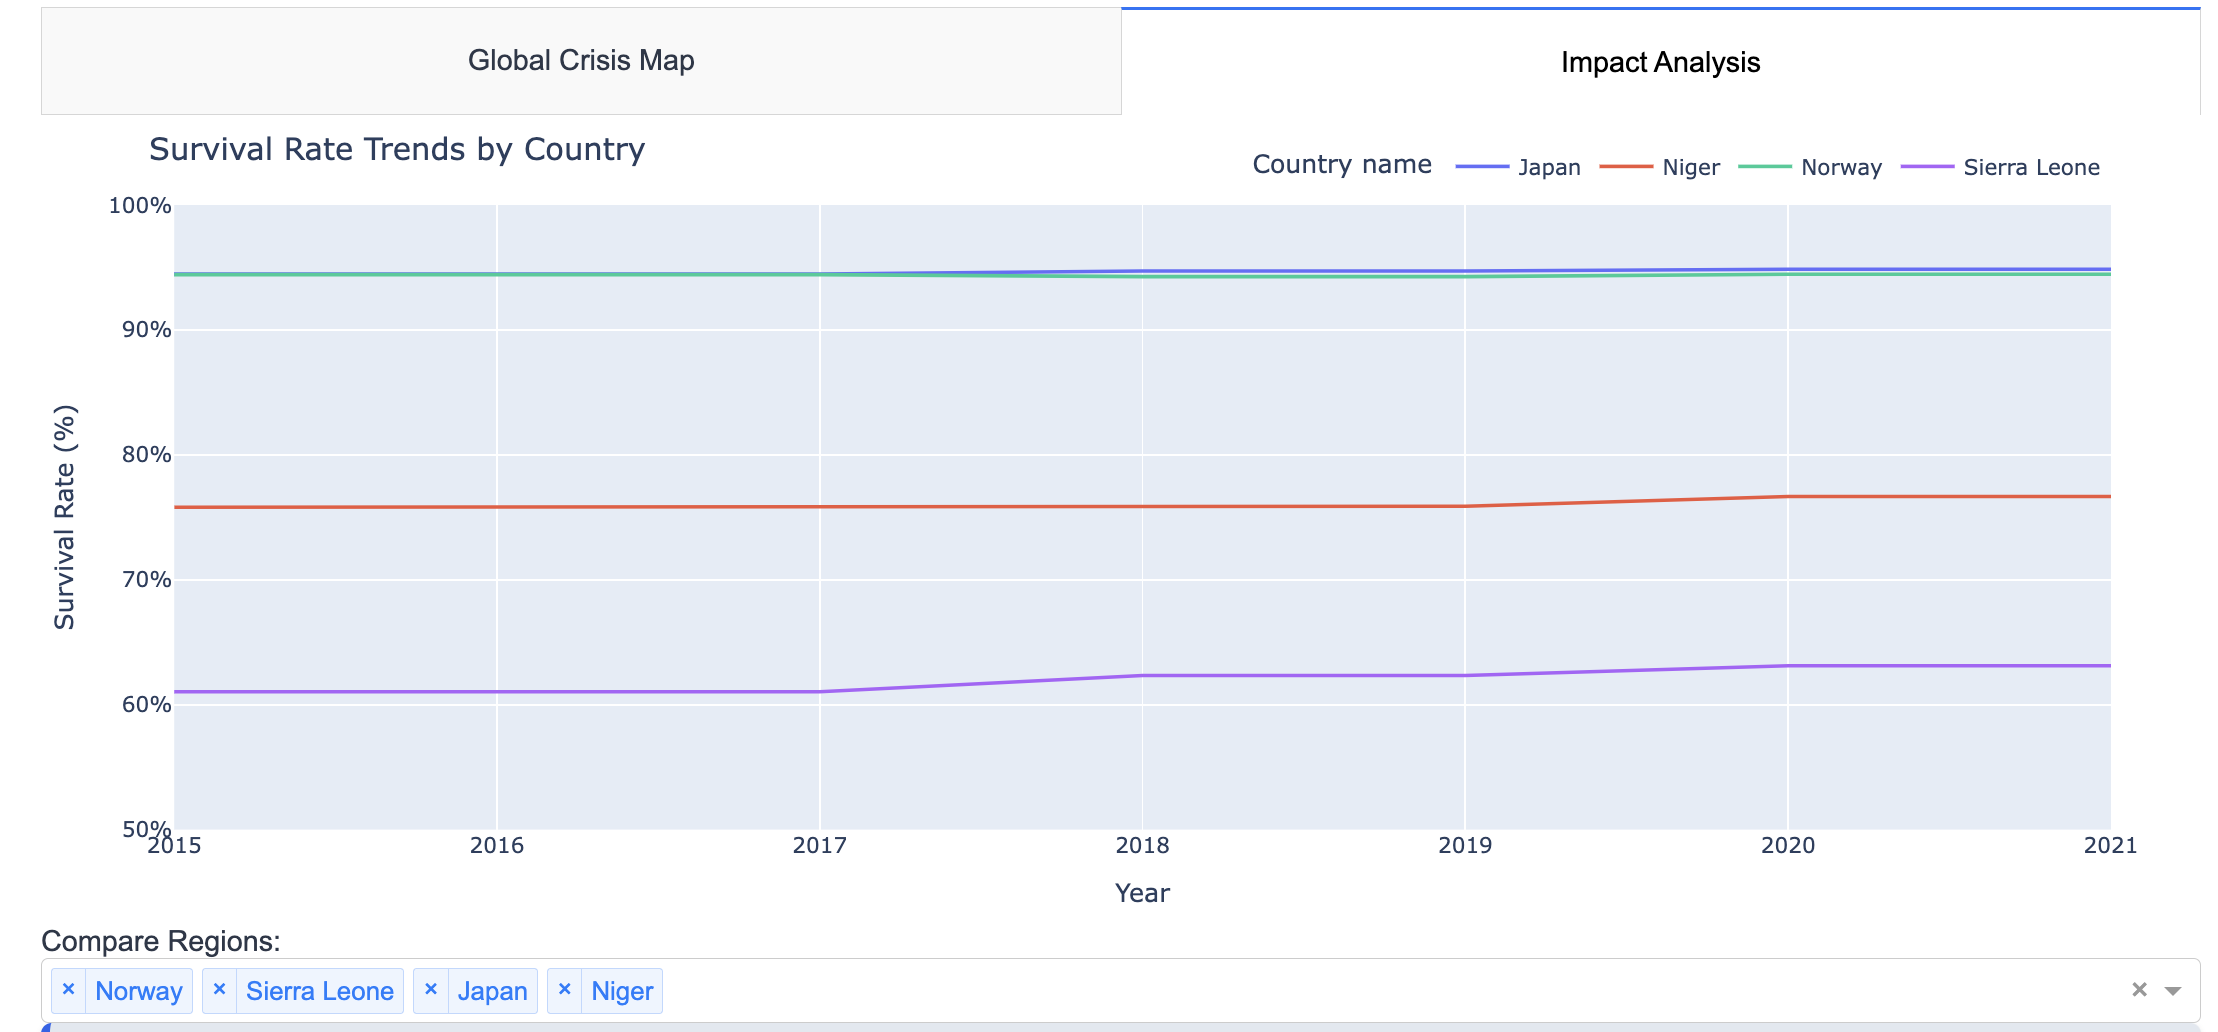
\includegraphics[width=\textwidth]{survival_rates.png}
    \caption{Survival Rate Comparison: Developed vs. Developing Nations (2015-2021). Showing the stark contrast between countries like Norway and Japan ($>$90\%) versus Sierra Leone and Niger ($<$ 70\%).}
    \label{fig:comparison}
\end{figure}

This stage demonstrates the gap between developed and developing nations through:
\begin{itemize}
    \item Interactive line chart comparing multiple countries
    \item Clear visualization of the ~30\% gap in survival rates
    \item Trend analysis over time
\end{itemize}

\subsection{Stage 3: Success Stories}
\begin{figure}[H]
    \centering
    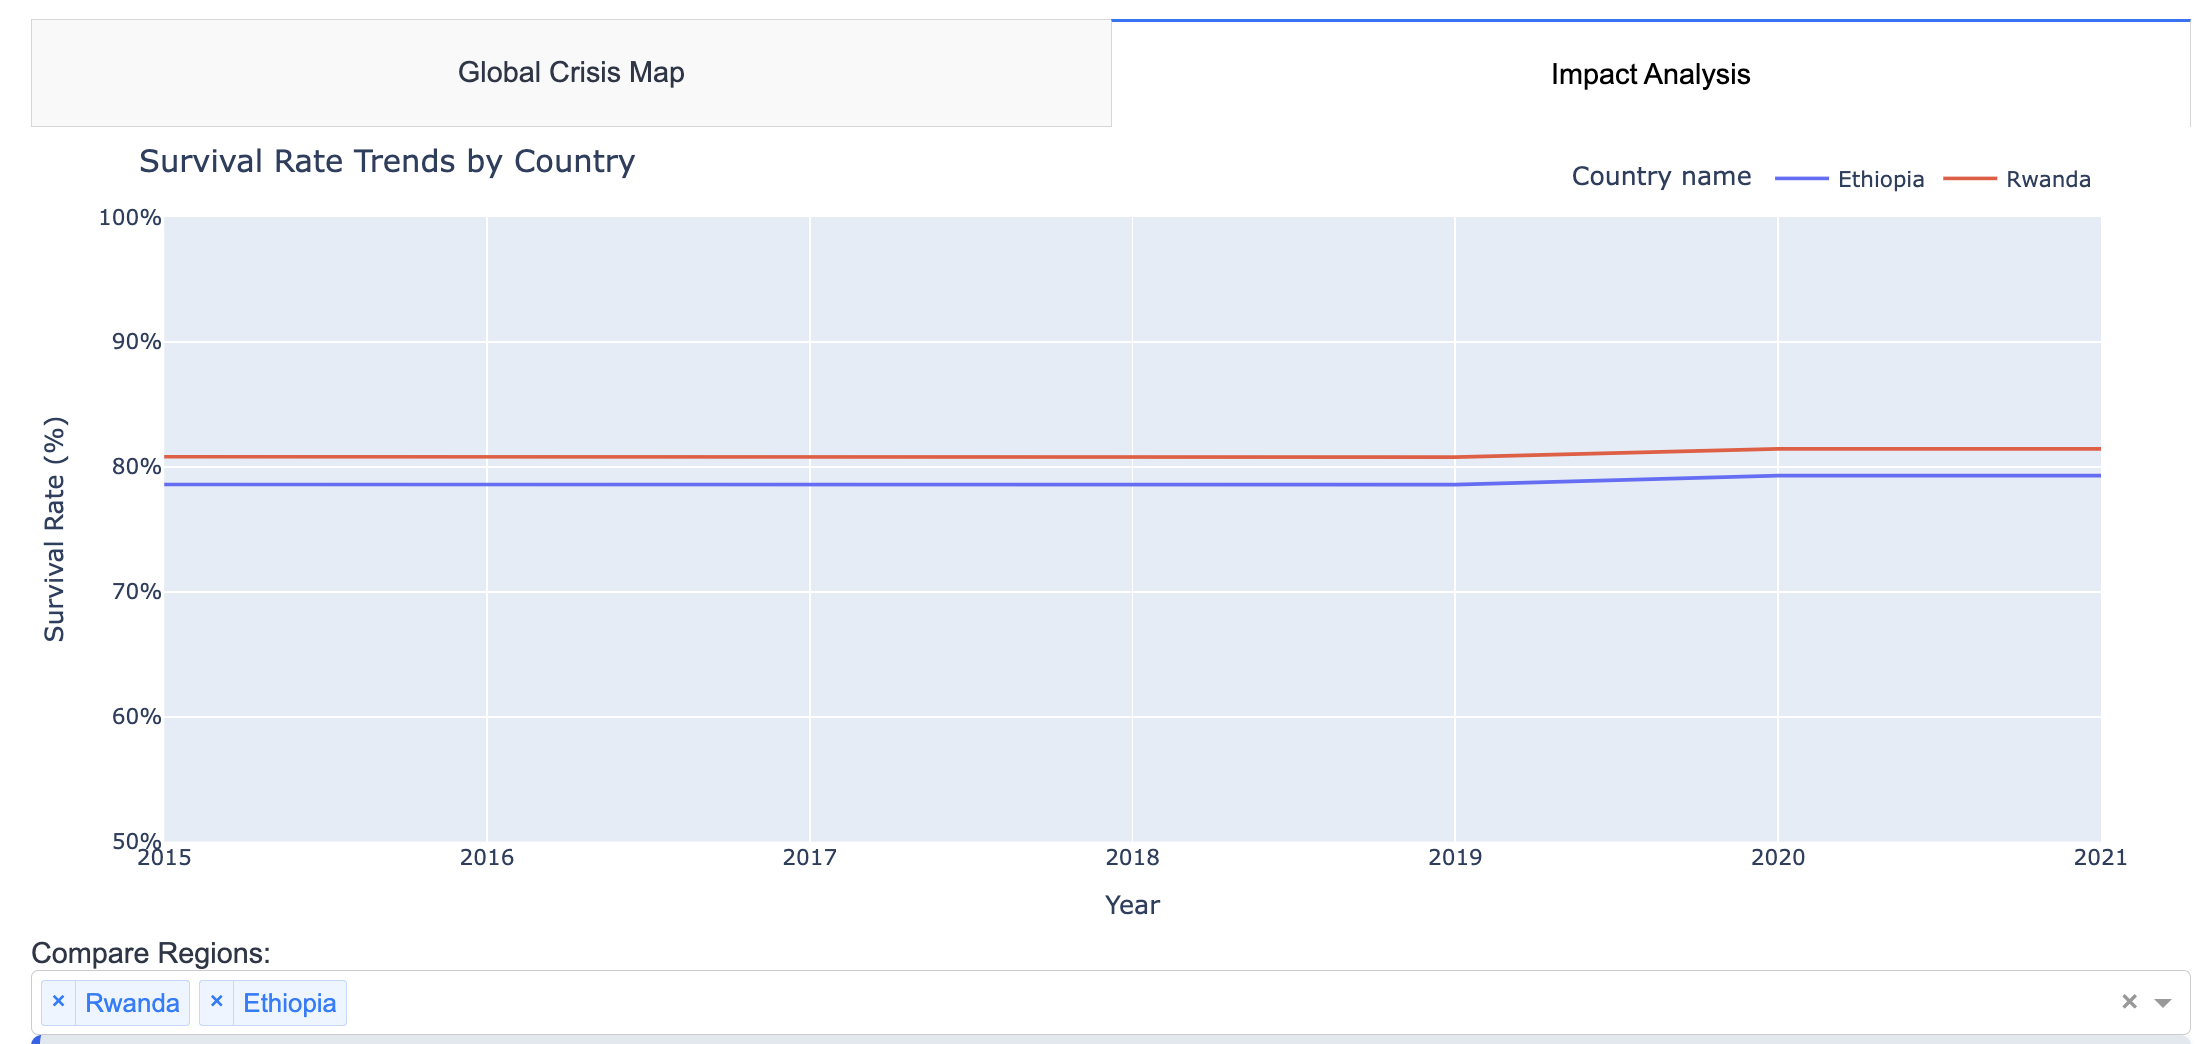
\includegraphics[width=\textwidth]{survival_rates2.png}
    \caption{Educational Investment Success Stories: Rwanda and Ethiopia showing steady improvements in survival rates through educational investment (2015-2021).}
    \label{fig:success}
\end{figure}
\section{Technical Implementation}
\subsection{Data Processing and Quality}
\begin{itemize}
    \item Robust handling of missing values using forward/backward fill
    \item Data validation ensuring values within expected ranges
    \item Quality checks for temporal consistency
    \item Error handling for edge cases
\end{itemize}

\subsection{Interactive Feature Implementation}
\begin{itemize}
    \item Real-time data updates without page reload
    \item Smooth transitions between narrative steps
    \item Coordinated updates across visualizations
    \item Responsive design for various screen sizes
\end{itemize}

\section{Critical Analysis}
\subsection{Strengths}
\begin{itemize}
    \item Intuitive navigation through complex data
    \item Clear visual hierarchy supporting narrative
    \item Multiple interaction paths for exploration
    \item Strong advocacy message supported by data
\end{itemize}

\subsection{Visualization Shortcomings}
\begin{itemize}
    \item \textbf{Technical Constraints}:
        \begin{itemize}
            \item Limited time range (2015-2021) restricts long-term trend analysis
            \item Some developing nations have incomplete data
            \item Map interactions can be slow during rapid year changes
        \end{itemize}
    \item \textbf{Design Limitations}:
        \begin{itemize}
            \item Color scheme may present challenges for colorblind users
            \item Small countries are difficult to select on the map
            \item Limited screen space optimization for mobile devices
        \end{itemize}
    \item \textbf{Narrative Elements}:
        \begin{itemize}
            \item Fixed story path limits free exploration
            \item Limited additional context about educational metrics
            \item No save/share functionality for specific views
        \end{itemize}
\end{itemize}

\subsection{Limitations and Future Work}
\begin{itemize}
    \item Limited time range (2015-2021)
    \item Some regions lack complete data
    \item Additional educational metrics could strengthen correlation
    \item Potential for more advanced statistical analysis
\end{itemize}
\section*{Extra Credit: Rhetorical Analysis}
\subsection*{Visualization Analysis: "Film Dialogue: Gender Distribution in Movies"}

\textbf{Source:} The Pudding's data visualization essay on gender representation in film dialogue

\subsection*{Narrative Structure and Persuasive Techniques}
The visualization employs several powerful rhetorical strategies:
\begin{itemize}
    \item \textbf{Progressive Disclosure}:
        \begin{itemize}
            \item Opens with a striking overall statistic
            \item Guides viewers through increasingly detailed analysis
            \item Builds evidence systematically through interactive elements
        \end{itemize}
    \item \textbf{Personal Connection}:
        \begin{itemize}
            \item Uses familiar movies to engage viewers
            \item Allows exploration of favorite films
            \item Makes abstract statistics tangible
        \end{itemize}
\end{itemize}

\subsection*{Visual Elements Supporting the Message}
\begin{itemize}
    \item \textbf{Color Coding}:
        \begin{itemize}
            \item Consistent blue/red scheme for gender identification
            \item Size of elements proportional to speaking time
            \item Clear visual hierarchy emphasizing disparities
        \end{itemize}
    \item \textbf{Interactive Features}:
        \begin{itemize}
            \item Scrollytelling format maintains engagement
            \item Interactive filters allow personal discovery
            \item Animated transitions emphasize key points
        \end{itemize}
\end{itemize}

\subsection*{Call to Action Effectiveness}
The visualization succeeds in:
\begin{itemize}
    \item Making inequity visible and measurable
    \item Providing clear evidence for industry change
    \item Encouraging audience awareness in media consumption
\end{itemize}

\subsection*{Ethical Considerations}
\begin{itemize}
    \item \textbf{Data Representation}:
        \begin{itemize}
            \item Transparent methodology
            \item Clear acknowledgment of limitations
            \item Balanced presentation of findings
        \end{itemize}
    \item \textbf{Potential Concerns}:
        \begin{itemize}
            \item Focus on mainstream Hollywood films
            \item Binary gender representation
            \item Limited historical context
        \end{itemize}
\end{itemize}

The visualization effectively advocates for gender equality in film through data-driven storytelling while maintaining ethical standards in data presentation. Its success lies in combining emotional resonance with rigorous analysis, making complex data accessible and actionable for viewers.
\end{document}